%%%%%%%%%%%%%%%%%%%%%%%%%%%%%%%%%%%%%%%%%%%%%%%%%%%%%%%%%%%%%%%%
% %
% Due Date %
% Andrew Gibson %
% ECE 351 lab, Section 53 %
% Lab 8 %
% Due 21 Mar 2023 %
% Step and Impulse Response of an RLC Bandpass Filter %
%https://github.com/gibs0630/ECE351\_Code %
%https://github.com/gibs0630/ECE351\_Reports %
% %
%%%%%%%%%%%%%%%%%%%%%%%%%%%%%%%%%%%%%%%%%%%%%%%%%%%%%%%%%%%%%%%%

\documentclass[12pt,a4paper]{article}
\usepackage[utf8]{inputenc}
\usepackage[greek,english]{babel}
\usepackage{alphabeta} 
\usepackage[pdftex]{graphicx}
\usepackage[top=1in, bottom=1in, left=1in, right=1in]{geometry}
\linespread{1.06}
\setlength{\parskip}{8pt plus2pt minus2pt}
\widowpenalty 10000
\clubpenalty 10000
\newcommand{\eat}[1]{}
\newcommand{\HRule}{\rule{\linewidth}{0.5mm}}
\usepackage[official]{eurosym}
\usepackage{enumitem}
\setlist{nolistsep,noitemsep}
\usepackage[hidelinks]{hyperref}
\usepackage{cite}
\usepackage{lipsum}

\newcommand{\Q}{\leavevmode\par\textbf {Q:}}
\newcommand{\A}{\par\textbf{A:} \normalfont}

\hypersetup{colorlinks=true, linkcolor=black, urlcolor=blue}

\begin{document}
%===========================================================
\begin{titlepage}
\begin{center}
% Top 
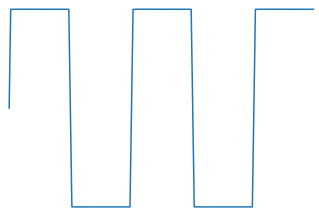
\includegraphics[width=0.55\textwidth]{titlepage_image.png}~\\[2cm]
% Title
\HRule \\[0.4cm]
{ \LARGE 
  \textbf{Project Report for ECE 351}\\[0.4cm]
  \emph{Lab 8: Fourier Series Approximation of a Square Wave}\\[0.4cm]
}
\HRule \\[1.5cm]
% Author
{ \large
  Andrew Gibson \\[0.1cm]
 28 February 2023\\[0.1cm]
  \url{https://github.com/gibs0630/ECE351\_Code}\\[0.1cm]
  \url{https://github.com/gibs0630/ECE351\_Reports}\\[0.1cm]
  %#\texttt{user@cut.ac.cy}
}
\vfill
%\textsc{\Large Cyprus University of Technology}\\[0.4cm]\textsc{\large Department of Electrical Engineering,\\Computer Engineering \& Informatics}\\[0.4cm]
% Bottom
{\large }
 
\end{center}
\end{titlepage}
%\begin{abstract}
%\lipsum[1-2]
%\addtocontents{toc}{\protect\thispagestyle{empty}}
%\end{abstract}
\newpage
%===========================================================
\tableofcontents
\addtocontents{toc}{\protect\thispagestyle{empty}}
\newpage
\setcounter{page}{1}
%===========================================================
%===========================================================
\section{Introduction}\label{sec:intro}
Fourier series allows for the construction of a function as a series of cosines and sines. Using python software, it is trivial to compute the summation of the cosines and sines using loop logic.

\section{Equations}\label{sec:lit-rev}
Formula's used
unit step function
\[
u(x) = \left\{
        \begin{array}{ll}
            0 & \quad t < 0 \\
            1 & \quad t \geq 0
        \end{array}
    \right.
\]
pulse function

\[P_{\tau} = u \left (t-\frac \tau 2 \right)-u \left (t+\frac \tau 2 \right)\]

Fourier's series
\[x(t) = \frac 1  2 a_0 + \sum_{k=1}^\infty \left[ a_k cos \left (k \frac {2\pi}  T t \right) + b_k sin \left(k \frac {2\pi}  T t \right) \right]\]

\[a_0 = \frac 2 T \int_0^T \left [ x_0(t) dt \right ]\]

\[a_k = \frac 2 T \int_0^T \left [ x_0(t) cos \left (k \frac {2 \pi} T t \right )dt \right ]\]

\[b_k = \frac 2 T \int_0^T \left [ x_0(t) sin \left (k \frac {2 \pi} T t \right )dt \right ]\]


equations from the lab

\[x_0(t) = 2 P_{\frac T 2} \left (t-\frac T 4 \right)- 1\]
\[a_k =  0\]
\[b_k =   \frac 2  {k \pi}   \left [ 1-(-1)^k \right ] \]


\[x(t) = \frac 2  { \pi }  \sum _{k=1}^\infty \left[ \left (\frac 1  {k}   \left [1- (-1)^k \right ] \right) sin \left(k \frac {2 \pi}  {T} t \right) \right]\]

\[x(t) = \frac 4  { \pi }  \sum_{n=1}^\infty \left[ \left(\frac 1  {2n-1}    \right) sin \left((2n-1) \frac {2 \pi} {T} t \right) \right]\]


\section{Methodology}\label{sec:meth}
This lab had us find the Fourier series by hand of a square wave.  We then used python to generate a signal of various sine waves and add them up to approximate the square wave as more terms in the summation are added.

\section{Results}\label{sec:res}
\subsection*{Part 1}



task 1\\
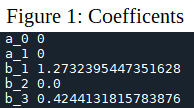
\includegraphics[width=0.25\textwidth]{Figure1.png}\\
Figure 1 shows the output of the various terms.

task 2\\
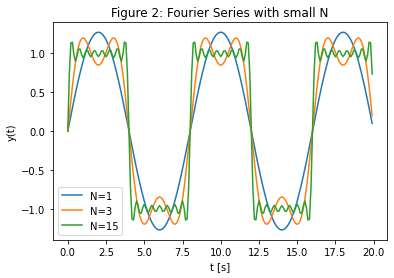
\includegraphics[width=0.55\textwidth]{Figure2.png}\\
Figure 2 shows that it makes a drastic difference when the first few terms are added.

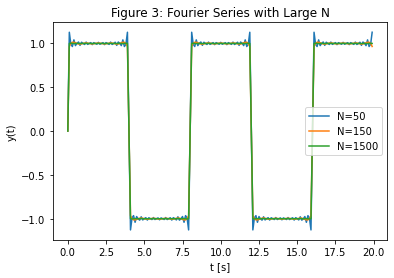
\includegraphics[width=0.55\textwidth]{Figure3.png}\\
Figure 3 shows that there is diminishing returns for a more and more accurate signal, and some artifacts(error) may appear on very small time intervals




\section{Questions}\label{sec:res}

\Q 1) Is x(t) an even or an odd function? Explain why. 
\A 1) x(t) is an odd function, because if you multiplied t by -1 and then multiplied the output by -1, you would get the original function.

\Q 2) Based on your results from Task 1, what do you expect the values of a$_2$, a$_3$, . . . , a$_n$ to be? Why?
\A 2) a$_k$ should be 0, because when solving for it, there were no other terms beside 0.

\Q 3) How does the approximation of the square wave change as the value of N increases? In what way does the Fourier series struggle to approximate the square wave?
\A 3) As the value of N increases, the wave becomes more and more square like and the plateaus and valleys become more and more flat. The Fourier series does struggle to get approximations at the impulse moments when it transitions from 1 to -1 and from -1 to 1.

\Q 4) What is occurring mathematically in the Fourier series summation as the value of N increases?
\A 4) As N increases, a more sine waves are being added to the output.

\Q 5) Leave any feedback on the clarity of lab tasks, expectations, and deliverables.
\A 5) For the periodic function used in this lab, a$_0$ and a$_k$ were 0, this caused confusion as the function a$_k$ for this case would always output 0. I would think that this lab would be better, or at least more clear on the what you are suppose to do on part 1 task 2, if we were to program the code that would take any function with a period (sequence of datapoints that would repeat outside of it's range), then the lab could have us "use" python to solve for a$_0$ and a$_0$ for any function period.
Also, the equations in the lab handout sheet do not distinguish between x$_0$ and x, where x$_0$ is the period of the function output of the period range.





%\lipsum[7-8]\cite{knuthwebsite}
%===========================================================
%===========================================================
\bibliographystyle{ieeetr}
\bibliography{refs}
\end{document} 
Annotations











